\subsection{Support-Vector-Machine}
Da es sich bei der Problemstellung um eine Klassifikation von zwei statischen Klassen handelt, ist der Einsatz einer Support-Vector-Machine (SVM) denkbar. Besonders die große Dimension der Merkmalsvektoren ist hierbei ein Grund zur Wahl einer SVM. In dieser Arbeit werden dabei der \glqq Radial Basic Function\grqq{} (RBF) Kernel sowie ein linearer Kernel verwendet.
Die in dieser Arbeit implementierte SVM wird mit Hilfe des Framework \textit{sklearn} umgesetzt. Um eine für die SVM möglichst aussagekräftige Statistik zu erhalten und die bestmöglichen Parameter zu ermitteln, erfolgt bei der Evaluation eine  Kreuzvalidierung. Zudem werden bei der Verwendung der \textit{sklearn}-SVM die Parameter $\gamma$ und $C$ variiert um ein Over- und Underfitting zu vermeiden.

Das Resultat zur Wahl der Parameter zeigt hierbei, dass bei einer Wahl des Paramaters $C=1$ und des zusätzlichen Parameters $\gamma = 0.0977$ für eine SVM mit RBF Kernel, bereits eine Genauigkeit (engl. \glqq Accuracy\grqq{} (ACC)) von ca. 99\% erreicht werden kann (siehe Abbildung \ref{fig:c_chooseSVM} und \ref{fig:gamma_chooseSVM}).

\begin{figure}[h!]
\centering
% This file was created by matplotlib2tikz v0.6.17.
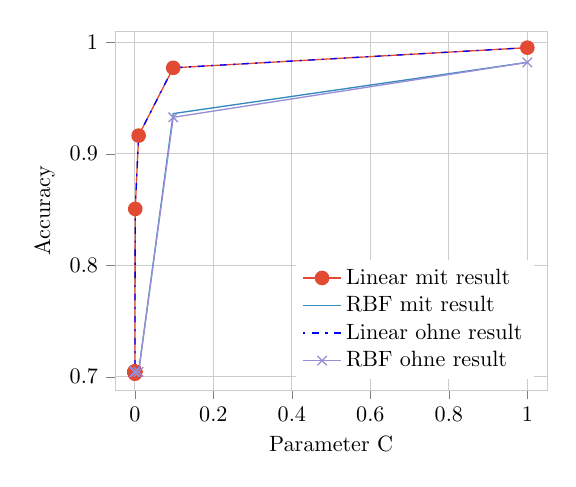
\begin{tikzpicture}[scale=.8,transform shape]

\definecolor{color0}{rgb}{0.886274509803922,0.290196078431373,0.2}
\definecolor{color1}{rgb}{0.203921568627451,0.541176470588235,0.741176470588235}
\definecolor{color2}{rgb}{0.596078431372549,0.556862745098039,0.835294117647059}

\begin{axis}[
xlabel={Parameter C},
ylabel={Accuracy},
xmin=-0.05, xmax=1.05,
ymin=0.688172131147541, ymax=1.00969672131148,
tick align=outside,
tick pos=left,
xmajorgrids,
x grid style={white!80.0!black},
ymajorgrids,
y grid style={white!80.0!black},
axis line style={white!80.0!black},
legend entries={{Linear mit result},{RBF mit result},{Linear ohne result},{RBF ohne result}},
legend cell align={left},
legend style={at={(0.97,0.03)}, anchor=south east, draw=none}
]
\addplot [semithick, color0, mark=*, mark size=3, mark options={solid}]
table {%
1e-100 0.704426229508197
1.02353102189903e-99 0.704426229508197
1.04761575278967e-98 0.704426229508197
1.07226722201033e-97 0.704426229508197
1.09749876549306e-96 0.704426229508197
1.12332403297803e-95 0.704426229508197
1.14975699539774e-94 0.704426229508197
1.176811952435e-93 0.704426229508197
1.20450354025879e-92 0.704426229508197
1.23284673944207e-91 0.704426229508197
1.26185688306603e-90 0.704426229508197
1.29154966501489e-89 0.704426229508197
1.32194114846604e-88 0.704426229508197
1.35304777457982e-87 0.704426229508197
1.38488637139389e-86 0.704426229508197
1.41747416292682e-85 0.704426229508197
1.45082877849595e-84 0.704426229508197
1.48496826225448e-83 0.704426229508197
1.51991108295295e-82 0.704426229508197
1.55567614393049e-81 0.704426229508197
1.59228279334111e-80 0.704426229508197
1.62975083462067e-79 0.704426229508197
1.66810053720008e-78 0.704426229508197
1.70735264747072e-77 0.704426229508197
1.74752840000771e-76 0.704426229508197
1.78864952905746e-75 0.704426229508197
1.8307382802954e-74 0.704426229508197
1.87381742286042e-73 0.704426229508197
1.91791026167252e-72 0.704426229508197
1.96304065004031e-71 0.704426229508197
2.00923300256509e-70 0.704426229508197
2.05651230834869e-69 0.704426229508197
2.10490414451206e-68 0.704426229508197
2.15443469003193e-67 0.704426229508197
2.20513073990309e-66 0.704426229508197
2.25701971963397e-65 0.704426229508197
2.31012970008318e-64 0.704426229508197
2.36448941264543e-63 0.704426229508197
2.4201282647944e-62 0.704426229508197
2.47707635599173e-61 0.704426229508197
2.53536449397014e-60 0.704426229508197
2.59502421139976e-59 0.704426229508197
2.65608778294672e-58 0.704426229508197
2.71858824273297e-57 0.704426229508197
2.78255940220716e-56 0.704426229508197
2.84803586843584e-55 0.704426229508197
2.91505306282522e-54 0.704426229508197
2.98364724028338e-53 0.704426229508197
3.05385550883341e-52 0.704426229508197
3.12571584968823e-51 0.704426229508197
3.19926713779738e-50 0.704426229508197
3.27454916287773e-49 0.704426229508197
3.35160265093885e-48 0.704426229508197
3.43046928631493e-47 0.704426229508197
3.51119173421514e-46 0.704426229508197
3.59381366380464e-45 0.704426229508197
3.67837977182865e-44 0.704426229508197
3.76493580679249e-43 0.704426229508197
3.85352859371055e-42 0.704426229508197
3.94420605943768e-41 0.704426229508197
4.03701725859658e-40 0.704426229508197
4.13201240011537e-39 0.704426229508197
4.22924287438953e-38 0.704426229508197
4.3287612810831e-37 0.704426229508197
4.43062145758392e-36 0.704426229508197
4.53487850812863e-35 0.704426229508197
4.64158883361283e-34 0.704426229508197
4.75081016210285e-33 0.704426229508197
4.86260158006541e-32 0.704426229508197
4.97702356433218e-31 0.704426229508197
5.09413801481645e-30 0.704426229508197
5.21400828799976e-29 0.704426229508197
5.33669923120639e-28 0.704426229508197
5.46227721768442e-27 0.704426229508197
5.59081018251231e-26 0.704426229508197
5.72236765935031e-25 0.704426229508197
5.85702081805677e-24 0.704426229508197
5.99484250318952e-23 0.704426229508197
6.13590727341329e-22 0.704426229508197
6.28029144183437e-21 0.704426229508197
6.42807311728445e-20 0.704426229508197
6.57933224657582e-19 0.704426229508197
6.73415065775097e-18 0.704426229508197
6.89261210434985e-17 0.704426229508197
7.0548023107188e-16 0.704426229508197
7.22080901838563e-15 0.704426229508197
7.39072203352596e-14 0.704426229508197
7.56463327554648e-13 0.704426229508197
7.74263682681147e-12 0.704426229508197
7.92482898353938e-11 0.704426229508197
8.11130830789709e-10 0.704426229508197
8.30217568131997e-09 0.704426229508197
8.49753435908668e-08 0.704426229508197
8.69749002617809e-07 0.704426229508197
8.90215085445065e-06 0.704426229508197
9.11162756115517e-05 0.702786885245902
0.000932603346883218 0.85051912568306
0.00954548456661833 0.916256830601093
0.0977009957299225 0.977021857923497
1 0.995081967213115
};
\addplot [semithick, color1, mark=asterisk*, mark size=3, mark options={solid}]
table {%
1e-100 0.704426229508197
1.02353102189903e-99 0.704426229508197
1.04761575278967e-98 0.704426229508197
1.07226722201033e-97 0.704426229508197
1.09749876549306e-96 0.704426229508197
1.12332403297803e-95 0.704426229508197
1.14975699539774e-94 0.704426229508197
1.176811952435e-93 0.704426229508197
1.20450354025879e-92 0.704426229508197
1.23284673944207e-91 0.704426229508197
1.26185688306603e-90 0.704426229508197
1.29154966501489e-89 0.704426229508197
1.32194114846604e-88 0.704426229508197
1.35304777457982e-87 0.704426229508197
1.38488637139389e-86 0.704426229508197
1.41747416292682e-85 0.704426229508197
1.45082877849595e-84 0.704426229508197
1.48496826225448e-83 0.704426229508197
1.51991108295295e-82 0.704426229508197
1.55567614393049e-81 0.704426229508197
1.59228279334111e-80 0.704426229508197
1.62975083462067e-79 0.704426229508197
1.66810053720008e-78 0.704426229508197
1.70735264747072e-77 0.704426229508197
1.74752840000771e-76 0.704426229508197
1.78864952905746e-75 0.704426229508197
1.8307382802954e-74 0.704426229508197
1.87381742286042e-73 0.704426229508197
1.91791026167252e-72 0.704426229508197
1.96304065004031e-71 0.704426229508197
2.00923300256509e-70 0.704426229508197
2.05651230834869e-69 0.704426229508197
2.10490414451206e-68 0.704426229508197
2.15443469003193e-67 0.704426229508197
2.20513073990309e-66 0.704426229508197
2.25701971963397e-65 0.704426229508197
2.31012970008318e-64 0.704426229508197
2.36448941264543e-63 0.704426229508197
2.4201282647944e-62 0.704426229508197
2.47707635599173e-61 0.704426229508197
2.53536449397014e-60 0.704426229508197
2.59502421139976e-59 0.704426229508197
2.65608778294672e-58 0.704426229508197
2.71858824273297e-57 0.704426229508197
2.78255940220716e-56 0.704426229508197
2.84803586843584e-55 0.704426229508197
2.91505306282522e-54 0.704426229508197
2.98364724028338e-53 0.704426229508197
3.05385550883341e-52 0.704426229508197
3.12571584968823e-51 0.704426229508197
3.19926713779738e-50 0.704426229508197
3.27454916287773e-49 0.704426229508197
3.35160265093885e-48 0.704426229508197
3.43046928631493e-47 0.704426229508197
3.51119173421514e-46 0.704426229508197
3.59381366380464e-45 0.704426229508197
3.67837977182865e-44 0.704426229508197
3.76493580679249e-43 0.704426229508197
3.85352859371055e-42 0.704426229508197
3.94420605943768e-41 0.704426229508197
4.03701725859658e-40 0.704426229508197
4.13201240011537e-39 0.704426229508197
4.22924287438953e-38 0.704426229508197
4.3287612810831e-37 0.704426229508197
4.43062145758392e-36 0.704426229508197
4.53487850812863e-35 0.704426229508197
4.64158883361283e-34 0.704426229508197
4.75081016210285e-33 0.704426229508197
4.86260158006541e-32 0.704426229508197
4.97702356433218e-31 0.704426229508197
5.09413801481645e-30 0.704426229508197
5.21400828799976e-29 0.704426229508197
5.33669923120639e-28 0.704426229508197
5.46227721768442e-27 0.704426229508197
5.59081018251231e-26 0.704426229508197
5.72236765935031e-25 0.704426229508197
5.85702081805677e-24 0.704426229508197
5.99484250318952e-23 0.704426229508197
6.13590727341329e-22 0.704426229508197
6.28029144183437e-21 0.704426229508197
6.42807311728445e-20 0.704426229508197
6.57933224657582e-19 0.704426229508197
6.73415065775097e-18 0.704426229508197
6.89261210434985e-17 0.704426229508197
7.0548023107188e-16 0.704426229508197
7.22080901838563e-15 0.704426229508197
7.39072203352596e-14 0.704426229508197
7.56463327554648e-13 0.704426229508197
7.74263682681147e-12 0.704426229508197
7.92482898353938e-11 0.704426229508197
8.11130830789709e-10 0.704426229508197
8.30217568131997e-09 0.704426229508197
8.49753435908668e-08 0.704426229508197
8.69749002617809e-07 0.704426229508197
8.90215085445065e-06 0.704426229508197
9.11162756115517e-05 0.704426229508197
0.000932603346883218 0.704426229508197
0.00954548456661833 0.704426229508197
0.0977009957299225 0.935983606557377
1 0.981912568306011
};
\addplot [semithick, blue, dash pattern=on 1pt off 3pt on 3pt off 3pt]
table {%
1e-100 0.704426229508197
1.02353102189903e-99 0.704426229508197
1.04761575278967e-98 0.704426229508197
1.07226722201033e-97 0.704426229508197
1.09749876549306e-96 0.704426229508197
1.12332403297803e-95 0.704426229508197
1.14975699539774e-94 0.704426229508197
1.176811952435e-93 0.704426229508197
1.20450354025879e-92 0.704426229508197
1.23284673944207e-91 0.704426229508197
1.26185688306603e-90 0.704426229508197
1.29154966501489e-89 0.704426229508197
1.32194114846604e-88 0.704426229508197
1.35304777457982e-87 0.704426229508197
1.38488637139389e-86 0.704426229508197
1.41747416292682e-85 0.704426229508197
1.45082877849595e-84 0.704426229508197
1.48496826225448e-83 0.704426229508197
1.51991108295295e-82 0.704426229508197
1.55567614393049e-81 0.704426229508197
1.59228279334111e-80 0.704426229508197
1.62975083462067e-79 0.704426229508197
1.66810053720008e-78 0.704426229508197
1.70735264747072e-77 0.704426229508197
1.74752840000771e-76 0.704426229508197
1.78864952905746e-75 0.704426229508197
1.8307382802954e-74 0.704426229508197
1.87381742286042e-73 0.704426229508197
1.91791026167252e-72 0.704426229508197
1.96304065004031e-71 0.704426229508197
2.00923300256509e-70 0.704426229508197
2.05651230834869e-69 0.704426229508197
2.10490414451206e-68 0.704426229508197
2.15443469003193e-67 0.704426229508197
2.20513073990309e-66 0.704426229508197
2.25701971963397e-65 0.704426229508197
2.31012970008318e-64 0.704426229508197
2.36448941264543e-63 0.704426229508197
2.4201282647944e-62 0.704426229508197
2.47707635599173e-61 0.704426229508197
2.53536449397014e-60 0.704426229508197
2.59502421139976e-59 0.704426229508197
2.65608778294672e-58 0.704426229508197
2.71858824273297e-57 0.704426229508197
2.78255940220716e-56 0.704426229508197
2.84803586843584e-55 0.704426229508197
2.91505306282522e-54 0.704426229508197
2.98364724028338e-53 0.704426229508197
3.05385550883341e-52 0.704426229508197
3.12571584968823e-51 0.704426229508197
3.19926713779738e-50 0.704426229508197
3.27454916287773e-49 0.704426229508197
3.35160265093885e-48 0.704426229508197
3.43046928631493e-47 0.704426229508197
3.51119173421514e-46 0.704426229508197
3.59381366380464e-45 0.704426229508197
3.67837977182865e-44 0.704426229508197
3.76493580679249e-43 0.704426229508197
3.85352859371055e-42 0.704426229508197
3.94420605943768e-41 0.704426229508197
4.03701725859658e-40 0.704426229508197
4.13201240011537e-39 0.704426229508197
4.22924287438953e-38 0.704426229508197
4.3287612810831e-37 0.704426229508197
4.43062145758392e-36 0.704426229508197
4.53487850812863e-35 0.704426229508197
4.64158883361283e-34 0.704426229508197
4.75081016210285e-33 0.704426229508197
4.86260158006541e-32 0.704426229508197
4.97702356433218e-31 0.704426229508197
5.09413801481645e-30 0.704426229508197
5.21400828799976e-29 0.704426229508197
5.33669923120639e-28 0.704426229508197
5.46227721768442e-27 0.704426229508197
5.59081018251231e-26 0.704426229508197
5.72236765935031e-25 0.704426229508197
5.85702081805677e-24 0.704426229508197
5.99484250318952e-23 0.704426229508197
6.13590727341329e-22 0.704426229508197
6.28029144183437e-21 0.704426229508197
6.42807311728445e-20 0.704426229508197
6.57933224657582e-19 0.704426229508197
6.73415065775097e-18 0.704426229508197
6.89261210434985e-17 0.704426229508197
7.0548023107188e-16 0.704426229508197
7.22080901838563e-15 0.704426229508197
7.39072203352596e-14 0.704426229508197
7.56463327554648e-13 0.704426229508197
7.74263682681147e-12 0.704426229508197
7.92482898353938e-11 0.704426229508197
8.11130830789709e-10 0.704426229508197
8.30217568131997e-09 0.704426229508197
8.49753435908668e-08 0.704426229508197
8.69749002617809e-07 0.704426229508197
8.90215085445065e-06 0.704426229508197
9.11162756115517e-05 0.702786885245902
0.000932603346883218 0.85051912568306
0.00954548456661833 0.916256830601093
0.0977009957299225 0.977021857923497
1 0.995081967213115
};
\addplot [semithick, color2, mark=x, mark size=3, mark options={solid}]
table {%
1e-100 0.704426229508197
1.02353102189903e-99 0.704426229508197
1.04761575278967e-98 0.704426229508197
1.07226722201033e-97 0.704426229508197
1.09749876549306e-96 0.704426229508197
1.12332403297803e-95 0.704426229508197
1.14975699539774e-94 0.704426229508197
1.176811952435e-93 0.704426229508197
1.20450354025879e-92 0.704426229508197
1.23284673944207e-91 0.704426229508197
1.26185688306603e-90 0.704426229508197
1.29154966501489e-89 0.704426229508197
1.32194114846604e-88 0.704426229508197
1.35304777457982e-87 0.704426229508197
1.38488637139389e-86 0.704426229508197
1.41747416292682e-85 0.704426229508197
1.45082877849595e-84 0.704426229508197
1.48496826225448e-83 0.704426229508197
1.51991108295295e-82 0.704426229508197
1.55567614393049e-81 0.704426229508197
1.59228279334111e-80 0.704426229508197
1.62975083462067e-79 0.704426229508197
1.66810053720008e-78 0.704426229508197
1.70735264747072e-77 0.704426229508197
1.74752840000771e-76 0.704426229508197
1.78864952905746e-75 0.704426229508197
1.8307382802954e-74 0.704426229508197
1.87381742286042e-73 0.704426229508197
1.91791026167252e-72 0.704426229508197
1.96304065004031e-71 0.704426229508197
2.00923300256509e-70 0.704426229508197
2.05651230834869e-69 0.704426229508197
2.10490414451206e-68 0.704426229508197
2.15443469003193e-67 0.704426229508197
2.20513073990309e-66 0.704426229508197
2.25701971963397e-65 0.704426229508197
2.31012970008318e-64 0.704426229508197
2.36448941264543e-63 0.704426229508197
2.4201282647944e-62 0.704426229508197
2.47707635599173e-61 0.704426229508197
2.53536449397014e-60 0.704426229508197
2.59502421139976e-59 0.704426229508197
2.65608778294672e-58 0.704426229508197
2.71858824273297e-57 0.704426229508197
2.78255940220716e-56 0.704426229508197
2.84803586843584e-55 0.704426229508197
2.91505306282522e-54 0.704426229508197
2.98364724028338e-53 0.704426229508197
3.05385550883341e-52 0.704426229508197
3.12571584968823e-51 0.704426229508197
3.19926713779738e-50 0.704426229508197
3.27454916287773e-49 0.704426229508197
3.35160265093885e-48 0.704426229508197
3.43046928631493e-47 0.704426229508197
3.51119173421514e-46 0.704426229508197
3.59381366380464e-45 0.704426229508197
3.67837977182865e-44 0.704426229508197
3.76493580679249e-43 0.704426229508197
3.85352859371055e-42 0.704426229508197
3.94420605943768e-41 0.704426229508197
4.03701725859658e-40 0.704426229508197
4.13201240011537e-39 0.704426229508197
4.22924287438953e-38 0.704426229508197
4.3287612810831e-37 0.704426229508197
4.43062145758392e-36 0.704426229508197
4.53487850812863e-35 0.704426229508197
4.64158883361283e-34 0.704426229508197
4.75081016210285e-33 0.704426229508197
4.86260158006541e-32 0.704426229508197
4.97702356433218e-31 0.704426229508197
5.09413801481645e-30 0.704426229508197
5.21400828799976e-29 0.704426229508197
5.33669923120639e-28 0.704426229508197
5.46227721768442e-27 0.704426229508197
5.59081018251231e-26 0.704426229508197
5.72236765935031e-25 0.704426229508197
5.85702081805677e-24 0.704426229508197
5.99484250318952e-23 0.704426229508197
6.13590727341329e-22 0.704426229508197
6.28029144183437e-21 0.704426229508197
6.42807311728445e-20 0.704426229508197
6.57933224657582e-19 0.704426229508197
6.73415065775097e-18 0.704426229508197
6.89261210434985e-17 0.704426229508197
7.0548023107188e-16 0.704426229508197
7.22080901838563e-15 0.704426229508197
7.39072203352596e-14 0.704426229508197
7.56463327554648e-13 0.704426229508197
7.74263682681147e-12 0.704426229508197
7.92482898353938e-11 0.704426229508197
8.11130830789709e-10 0.704426229508197
8.30217568131997e-09 0.704426229508197
8.49753435908668e-08 0.704426229508197
8.69749002617809e-07 0.704426229508197
8.90215085445065e-06 0.704426229508197
9.11162756115517e-05 0.704426229508197
0.000932603346883218 0.704426229508197
0.00954548456661833 0.704426229508197
0.0977009957299225 0.932650273224044
1 0.981912568306011
};
\end{axis}

\end{tikzpicture}
\caption{\em Wahl des Parameter C mit Hilfe einer Kreuzvalidierung für eine SVM mit linearem und RBF Kernel}
\label{fig:c_chooseSVM}
\end{figure}

\begin{figure}[h!]
\centering
% This file was created by matplotlib2tikz v0.6.17.
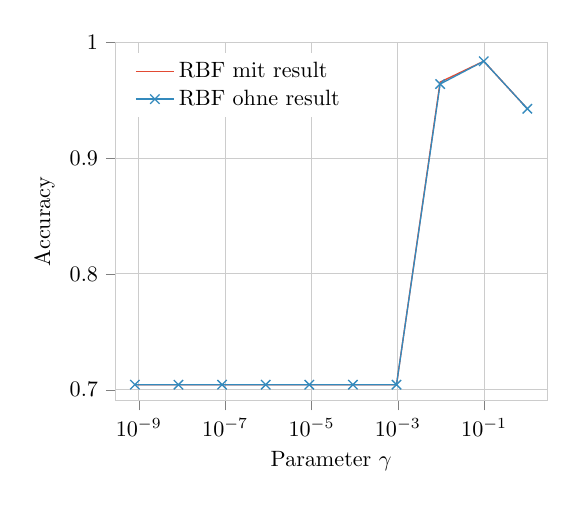
\begin{tikzpicture}[scale=.8,transform shape]

\definecolor{color0}{rgb}{0.886274509803922,0.290196078431373,0.2}
\definecolor{color1}{rgb}{0.203921568627451,0.541176470588235,0.741176470588235}

\begin{axis}[
xlabel={Parameter $\gamma$},
ylabel={Accuracy},
xmin=2.84803586843589e-10, xmax=2.8480358684358,
ymin=0.690468579234973, ymax=1.0,
xmode=log,
tick align=outside,
tick pos=left,
xmajorgrids,
x grid style={white!80.0!black},
ymajorgrids,
y grid style={white!80.0!black},
axis line style={white!80.0!black},
legend entries={{RBF mit result},{RBF ohne result}},
legend cell align={left},
legend style={at={(0.03,0.97)}, anchor=north west, draw=none}
]
\addplot [semithick, color0, mark=asterisk*, mark size=3, mark options={solid}]
table {%
8.11130830789709e-10 0.704426229508197
8.30217568131997e-09 0.704426229508197
8.49753435908668e-08 0.704426229508197
8.69749002617809e-07 0.704426229508197
8.90215085445065e-06 0.704426229508197
9.11162756115517e-05 0.704426229508197
0.000932603346883218 0.704426229508197
0.00954548456661833 0.96551912568306
0.0977009957299225 0.983579234972678
1 0.942540983606558
};
\addplot [semithick, color1, mark=x, mark size=3, mark options={solid}]
table {%
8.11130830789709e-10 0.704426229508197
8.30217568131997e-09 0.704426229508197
8.49753435908668e-08 0.704426229508197
8.69749002617809e-07 0.704426229508197
8.90215085445065e-06 0.704426229508197
9.11162756115517e-05 0.704426229508197
0.000932603346883218 0.704426229508197
0.00954548456661833 0.963879781420765
0.0977009957299225 0.983579234972678
1 0.942540983606558
};
\end{axis}

\end{tikzpicture}
\caption{\em Wahl des Parameter $\gamma$ mit Hilfe einer Kreuzvalidierung für eine SVM mit linearem und RBF Kernel}
\label{fig:gamma_chooseSVM}
\end{figure}
